\chapter{Methods}\label{methods}

\section {Participants and stimuli}

\subsection{Participants}

18 children and 22 adults were recruited from the internal participants database.
Subjects were selected if they spoke German as native language, if their language development was unremarkable, if their handedness score was above 70, if they fulfilled the prerequisites for MRI scans, and if their medical history was free of cognitive abnormalities.
4 children and 4 adults dropped out inbetween sessions of the study.
Two children were excluded from the analysis because their behavioral performance was at chance level.
12 children (5 female) and 18 adults (9 female) were left for the subsequent analysis.
Children were aged between 9y11m and 10y9m and described as right-handed by their parents.
Adults were aged between 22 and 33 years and scored between 73 to 100 (median: 95) on the laterality quotient test \cite{3.1.LQ}.
The point of reference for these ages is the time of the MEG session.
Parents gave written informed consent and were compensated with 40\euro \ for the MEG session and 7,50\euro \ for the MRI session.
Children agreed to participate in the study and were compensated with a 10\euro \ gift voucher for each session.
Adult participants were compensated with 20\euro.
All experimental procedures were approved by the University of Leipzig Ethical Review Board.


\subsection{Task}

The study consisted of two sessions: an anatomical MRI acquisition (duration: 50 minutes) and an interactive magnetoencephalographic measurement (typical duration: 90 minutes).
Since they took place in two different locations, there was a delay (median: 98 days, maximum: 243 days) between the two sessions.

The MRI session is described in detail in section 3.2.2.

The MEG session consisted of two sections: a tutorial section and a main section.

\paragraph{MEG tutorial section}

First, the tutorial section described the usage of the interface.

Second, subjects needed to respond to an example stimulus with the spoken sentence written out below the screen.

Third, three example trials followed without the written sentence.

Fourth, an artificially incomprehensible sentence was presented together with otherwise innocuous visual stimuli.

When subjects pressed either response button instead of skipping the trial, they were instructed with the skip function.

Finally, a series of randomized tutorial trials followed.
When subjects showed behavioral proficiency of the task, the tutorial ended prematurely.
Two thresholds for proficiency were possible: either an average response time below 3000ms and an accuracy score above 80\%, or an accuracy score above 88\%.
Either threshold could only be reached after completing at least 5 or 8 trials, respectively.
When none of these thresholds were met, the tutorial ended after 36 trials.

\paragraph{MEG main section}
The main section was used for MEG acquisition and consisted of 304 trials grouped in two blocks.
There was a scheduled break between the blocks (usually 1-2 minutes) which included interaction with the research assistant.
Subject-specific trial randomization was performed before the task.
All stimuli-related randomization tasks were implemented with a time-seeded Mersenne-Twister approach in Python 2.7.
Randomization contained two exceptions: neither the same image nor the same sentence could be played twice in a row.
Each block consisted of 8 clusters.
Subjects were shown a feedback screen at the end of each cluster, summarizing their performance throughout the recent cluster.
Since manual intervention was necessary to proceed to the next cluster, subjects frequently used this opportunity for a tiny break (typically 5-20 seconds).
Each cluster consisted of 19 trials.

\paragraph{Structure of a single trial}
Each trial started by showing two pictures side-by-side.
In one picture, one of the animals performs a social action on the other animal.
In the other picture, the roles are reversed.
10ms later, the spoken question started playing.
The subject could respond by pressing one of the direction buttons or the skip button.
There were two direction buttons, left or right, signifying that the left or right image contained the answer to the question.
The skip button was used to mark the trial as invalid for further analysis, and excluded the trial from performance feedback.
This response was the correct choice when the subject was distracted or failed to comprehend the question immediately.
This opened a minor pitfall: subjects could have gotten perfect scores by just pressing the skip button each time.
Fortunately, none of the subjects discovered this opportunity.
The trial ended with an auditory and visual feedback.


\subsection{Visual stimuli}

\paragraph{Character motivation}
A set of visual stimuli consisted of a two side-by-side images on black background.
Each image depicted two different animals on a white background.
I selected selected social activities that were only plausible for antropomorphised characters, not for their real animal counterparts.
Antropomorphization includes the use of their front limbs for object manipulation and standing on their hindlegs.
These measures are introduced to prevent associations with real-world animalistic behavior.
For example, a lion "'catching"' a monkey could resemble predatory behavior.
This association with chasing and killing would introduce a semantic bias against the reverse interaction: a real-life monkey "'catching"' a lion is much more implausible than the reverse.
To further detract from a naturalistic view, the animals were represented in a cartoon style.
To prevent unnecessary stress on this interpretation, I only selected animals whose real-life counterparts were approximately equally sized.

\begin{figure}[h]
\begin{center}
\vspace{7mm}
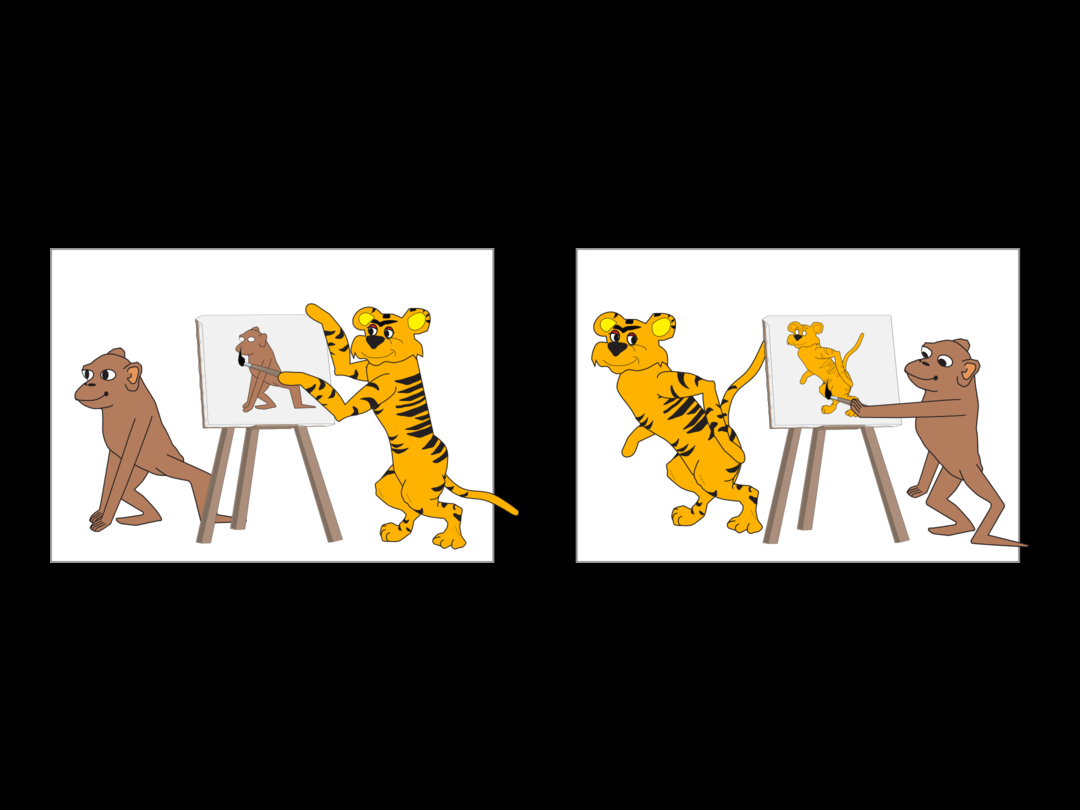
\includegraphics[width=0.5\textwidth]{pics/3_1_screen}
\caption{\label{3.1.screen} A typical visual stimulus, featuring two pairs of animals.}
\end{center}
\end{figure}

Image components were adapted with permission and kind advice from \cite{3.1.animals}.
Modifications were performed with Inkscape.

\begin{figure}[h]
\begin{center}
\vspace{7mm}
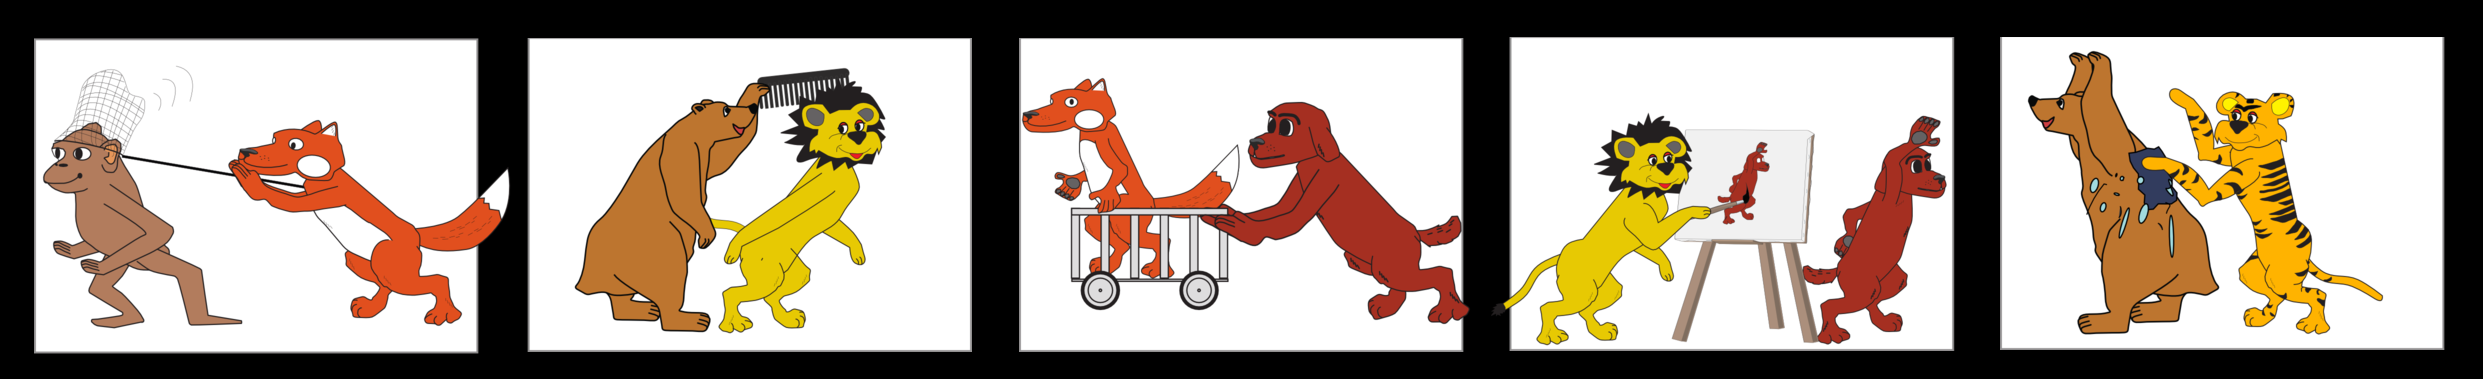
\includegraphics[width=0.99\textwidth]{pics/3_1_activities}
\caption{\label{3.1.activities} Illustrations of all five animals performing their social activities. From left to right: catching, combing, pushing, painting and washing}
\end{center}
\end{figure}

\paragraph{Trial feedback}
Immediately after each response, an icon appeared below one of the two displayed animal pairs.
The presented side was determined by the subject's response.
In the case of the skip button, the icon appeared at the same height as the others, but in the middle of the screen.
A green checkmark, a diagonal red cross and a yellow skip symbol signified a correct response, an incorrect response and an invalid trial, respectively.
The trial feedback screen was presented for a random interval between 400ms and 800ms.

\begin{figure}[h]
\begin{center}
\vspace{7mm}
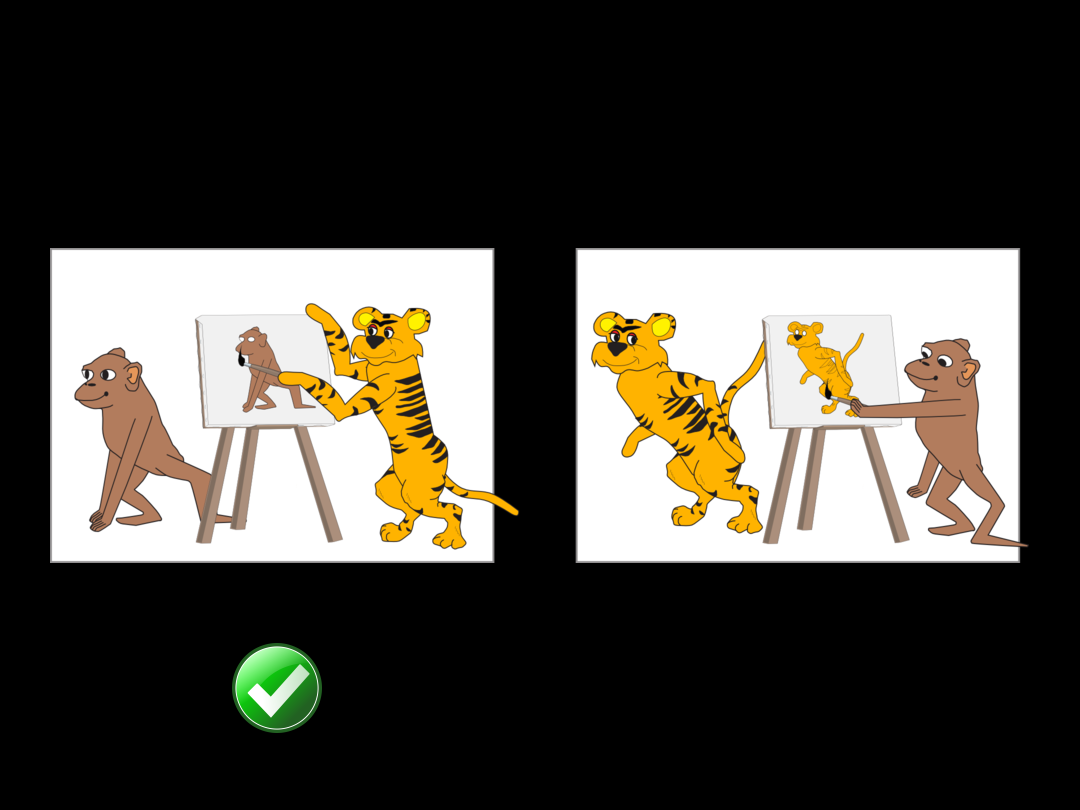
\includegraphics[width=0.5\textwidth]{pics/3_1_feedback}
\caption{\label{3.1.feedback} The visual feedback to a correct response.}
\end{center}
\end{figure}

\paragraph{Cluster feedback}
In this experiment, there was an obvious tradeoff between speed and accuracy.
To encourage a high level of attention and a high number of usable trials, two bar graphs visualized performance speed and accuracy (see Fig. \ref{3.1.clusterfeedback}).
In order to maximize the amount of usable trials for further analysis, the visualization valued accuracy much more than response time (see Fig. \ref{3.1.feedbackGraphs}).

\begin{figure}[h]
\begin{center}
\vspace{7mm}
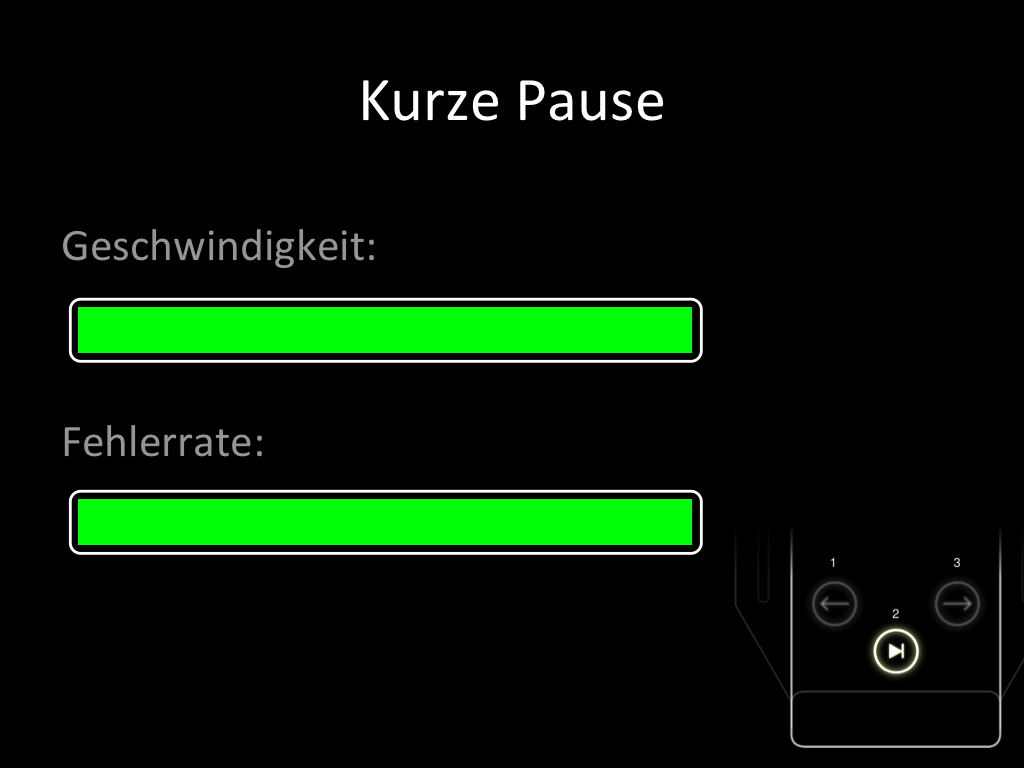
\includegraphics[width=0.5\textwidth]{pics/3_1_clusterfeedback}
\caption{\label{3.1.clusterfeedback} An ideal cluster feedback screen that appears after completing 19 trials. Upper bar: speed, lower bar: accuracy. Bottom right: indicator to  press the skip button to advance}
\end{center}
\end{figure}

\begin{figure}[h]
\begin{center}
\vspace{7mm}
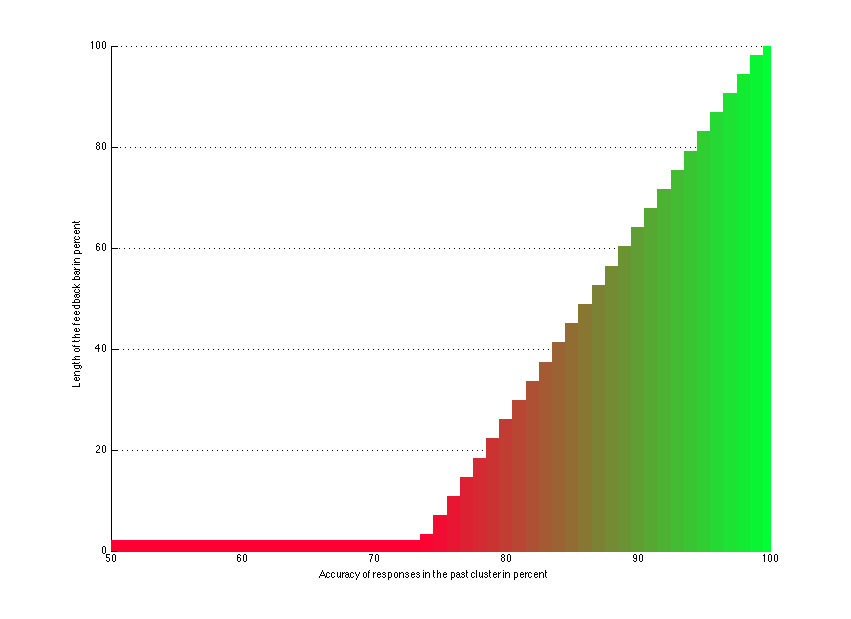
\includegraphics[width=0.45\textwidth]{pics/3_1_feedbackGraphAccuracy}
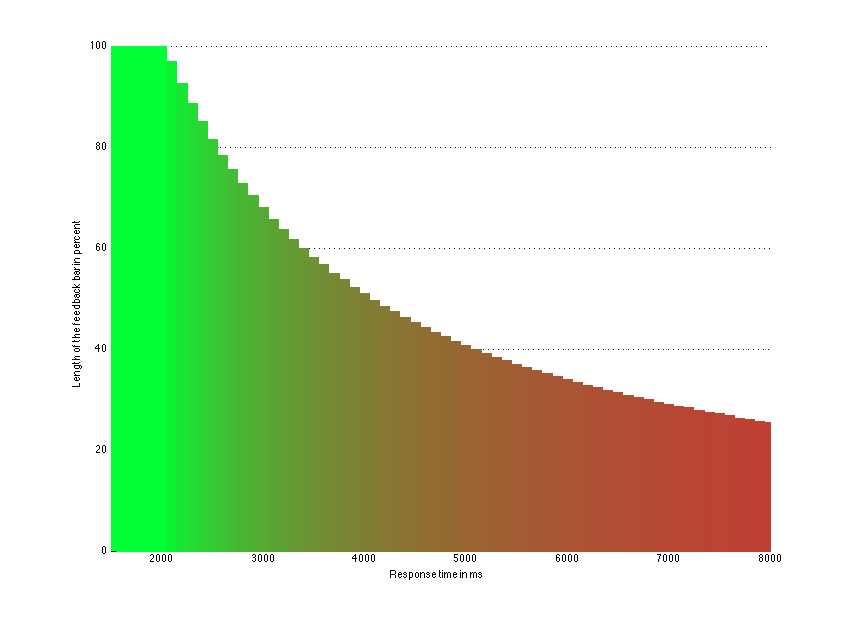
\includegraphics[width=0.45\textwidth]{pics/3_1_feedbackGraphRT}
\caption{\label{3.1.feedbackGraphs} Relation between performance and displayed feedback bars. Performance (left: RA, right: RT) is drawn along the X-axis, and length of the bars in \% is drawn along the Y-Axis.}
\end{center}
\end{figure}

\subsection{Auditory stimuli}

\paragraph{Sentence content}
Each pair of images was presented with a spoken question.
The question format fit well with the stimulus-response paradigm, and allowed the sentences to be identical until the conditional article ("'den"' or "'der"') appeared.
Syntactically, the sentences used an equal number of subject-relative and object-relative clauses.
In order to minimize confounding effects, these two conditions were designed to show as little auditory distinction as possible.
The structure of the final sentences is displayed in table \ref{3.1.sentences}.

\begin{table}[htb]
\vspace{5mm}
\begin{center}
\begin{tabular}{c|cccccccc}
Original & Wo & ist & das & Tier, & das & der & Tiger & malt?\\
Translated & Where & is & the & animal$_{OBJ}$, & which & the$_{NOM}$ & tiger$_{SUBJ}$ & paints?\\
Word index & 1 & 2 & 3 & 4 & 5 & 6 & 7 & 8
\end{tabular}
\caption{\label{3.1.sentences} Example stimulus sentence. Top: original spelling in German. Middle: Literal translation in English. Bottom: Word index within the sentence.}
\end{center}
\end{table}

\paragraph{Tutorial sentences}
During the pilot study, children often assumed that the every sentence was a subject-relative construction, miscategorizing "'den"' for "'der"'.
Tutorial sentences made the two animal nouns explicit, so that all sentences were structured in the format "'Where is the monkey that is caught by the dog?"'.
While this setup was creating strong auditory differences, it was easier to comprehend.
If the children didn't notice the difference by the eighth tutorial trial, the research assistant repeated the question with an exaggerated "'den"' pronounciation.

\paragraph{Audio format}
Sentences were spoken by a professional female native speaker in an uni\-so\-nous and moderately child-directed prosody.
Recording and playback was performed at a sampling rate of 44100Hz with one channel.
Loudness of each sentence was normalized.
Overall loudness was adjusted to 50db above each subject's individual hearing threshold.

\paragraph{Trial feedback}
Immediately after each response, one of two short sounds played.
The sounds were extracted from Microsoft Windows XP.
The "'external device plugged in"' icon (two bell sounds in ascending tone) and the "'external device removed"' icon (two bell sounds in descending tone) represented correct and incorrect responses, respectively.
No sound was played after the skip button.

\subsection{Experimental setup}
The participants were seated on a comfortable chair, inside a shielded, dimly-lit cabin.
Visual and auditory stimuli were produced by a computer running Presentation (version 14.0) at 60Hz refresh rate and 1024x768 resolution.
Video signal was routed through a video splitter MSV1235 into a Panasonic PT-D7700 projector.
Audio signals were generated by a Soundblaster Audigy 2 ZS [SB0350].
An audio amplifier (Compumedics, Hamburg, Germany) drove a pair of TIP-300 loudspeakers (Nicolet, Biomedical Madison, WI, U.S.A.).
Sound was routed through a pair of plastic tubes (50cm length, approx. delay of 1.6ms)
Sound arrived in the subjects' ears via ER3-14A/B earplugs (Etymotic Research Inc., Elk Grove Village IL, U.S.A.).

\section{Data acquisition}

\subsection {MEG}
MEG data were collected with an Elekta Neuromag VectorView\textsuperscript{\textregistered} MEG scanner in Bennewitz, at the development unit for Magnetoencephalography and Cortical Networks, Institute for Cognitive and Brain sciences, Leipzig, Germany.
The scanner comprised 306 MEG-channel sensors (102 magnetometers, 204 planar gradiometers).
Sensors were tuned prior to each MEG recording session to limit noise levels to approximately $2.5 \frac{fT\sqrt{Hz}}{cm}$.
Sensors that became very noisy during a recording block would be individually re-tuned at the next inter-block break, either by using the fine-tuning options or the selective heating function.
Continuous MEG data were recorded at 1000 Hz sampling rate (330 Hz lowpass filter).

Prior to data acquisition, all metal and other potential sources of electromagnetic interference were removed from participants.
Quality of recording was confirmed by visual inspection of a live view of MEG recording before each session without the subject present.
Electro-oculogram (EOG) and electrocardiogram (ECG) time-series were recorded simultaneously with MEG to track potential noise sources and artifacts.
Five head position indicator (HPI) coils were attached to the participant's forehead and a Polhemus stylus and digitizer device were used to record the locations of fiducial points (right and left pre-auricular points (RPA, LPA) and nasion), the HPI coils, and between 150 and 200 extra digitizer points on the head surface.
Prior to the recording of each stimulus block, head location in the scanner was measured with an automatic process that detected the coils.
Continuous HPI recorded any head movements during data acquisition.

\subsection {MRI}
Anatomical magnetic resonance imaging (aMRI) data were collected with a 3.0 Tesla TIM Trio scanner, located at the Max-Planck-Institute for Cognitive and Brain sciences.
Two scans were acquired from each participant in one session: A T1-weighted scan and a T2-weighted scan.
The T1-weighted scan used the magnetization-prepared rapid gradient echo (MPRAGE, \cite{3.2.mprage}]) sequence (flip angle = $9\textdegree$, TR/TE/TI = $2300ms/2.96ms/900ms$).
This scan was oriented transverse (176 slices) with an isotropic resolution of 1mm.
The T2-weighted scan used the SPACE sequence by \cite{3.2.space} (flip angle = $120\textdegree$, TR/TE = $3200ms/402ms$).
This scan was oriented transverse (176 slices at 1mm) with an inplane resolution of 0.5mm x 0.5mm.
All scans used a 32-channel head coil for the acquisition.


\section{Data analysis}

Data were preprocessed with the three software packages: Elekta Neuromag\textsuperscript{\textregistered} MaxFilter (version 2.2, \cite{3.3.MNE}), Matlab (version 2014a) and MNE-Python (version 0.8.6, \cite{3.3.MNEpython}).

\subsection{Behavioral data}

Two types of behavioral data were analyzed for group and condition effects: response time (RT) and response accuracy (RA).
Response time was measured at the condition onset, i.e. at the "'d"' sound of "'den"' or "'der"' (in the subject-relative clause or the object-relative clause, respectively).
Trials were omitted when the subject skipped or answered them incorrectly.
Trials were also omitted if the response took longer than 4000ms.
This procedure removed 11.1\% of the childrens' trials, and 2.5\% of the adults' trials.

RT and RA were determined for each subject separately from the remaining trials.
Both metrics were tested for the requirements for an analysis of variance (ANOVA).
Normality of the residuals was tested with a Shapiro-Wilk test \cite{3.3.swtest}, implemented in Matlab.
Equality of variances was tested with a Levene test\cite{3.3.levtest}, implemented in SPSS.
RA data failed the normality test.
To include RA data in the following analysis, they were transformed to fit a normal distribution.
This transformation was accomplished with the inverted sigmoid function:
\[ \hat{a} = - log( \frac{1}{a} - 1 ) \]
All results from the ANOVA were transformed back into milisecond space with the sigmoid function:
\[ r = \frac{1}{1+e^{-\hat{r}}} \]


\subsection{Sensor-space activity}

\paragraph{Preprocessing and HPI correction}
Signal-space separation \cite{3.3.SSS} was used to reduce noise in the data by suppressing magnetic interference coming from outside and inside the sensory array.
MEG recordings were corrected for HPI movements, and co-registered across blocks to the inital head position for each individual.
All of these steps were computed with MaxFilter.
Data were then subjected to a 0.4Hz FIR highpass filter (Hamming window design, 4367 coefficients, -130db suppression at 0Hz, -3db at 0.4Hz,processing in Matlab) to remove slow trends.

\paragraph{Artifact removal}
MEG channels with abnormally high noise levels as identified by visual inspection were rejected from further analysis. A median of 1 channel (maximum: 3 channels) was removed.
The resulting pre-processed data contained major artifacts from spontaneous channel jumps, electrocardiographic (ECG) activity and electrooculographic (EOG) activity.
Jump amplitudes were detected by selecting peaks in the z-transformed continuous data that exceeded a threshold of 12 standard deviations.
Segments of 2 seconds in the pre-processed continuous data were rejected if any magnitude channel exceeded an amplitude of $6\cdot10^{-12}T$ (gradiometer channels: $4\cdot10^{-12}\frac{T}{cm}$).
Continuous data were then decomposed into independent components (ICA) that explained 99\% of the variance.
Components that correlated with EOG or ECG channels were removed with the MNE methods $preprocessing.ica\_find\_ecg\_events()$ and $preprocessing.ica\_find\_eog\_events()$, respectively.
ICA-based correction removed an average of 2.1 components per subject and block (minimum: 1, maximum: 4).
The remaining ICA components were used to reconstruct continuous data.

\paragraph{Epoching}
The main trigger was set at the condition onset (described in section 3.1.4).
Epochs were created between 1000ms before and 4000ms after the main trigger.
An epoch was rejected if the trial was skipped, or answered too slow (more than 4000ms) or answered incorrectly.
This procedure yielded an average of [] trials in children and [] trials in adults.
Data were filtered before epoching with a 45Hz FIR lowpass for visualization purposes only.

\paragraph{Establishing time windows of interest}
The condition effect was used to determine suitable time windows.
Selecting data purely based on contrast will include spurious differences as well as the condition-based differences in activity.
Since there the subsequent statistical analysis compares the same contrast, it is prone to overestimate the condition effect.
This problem was resolved with a cluster-level permutation comparison.
Spurious differences in activity should vary randomly between trials and subjects, while the condition contrast is expected with a roughly equal delay and duration.
Since the group had a strong impact on RT (see [4.1.1]), effective time windows were estimated separately for children and adults.

First, the mean was computed for data from all trials, separately for each subject and condition.

Second, sensor data was pooled by calculating the mean within each of three sensor groups (from parietal, temporal and frontal locations).
These locations were selected according to previous literature findings.
Finally, clusters were computed by the MNE function $stats.permutation\_cluster\_test()$ \cite{3.3.clustertest}.
The function was run with 500 permutations, and an t-threshold of 2.0.

For visualization purposes, grand average activity was also calculated for each sensor group and condition, separately for children and adults.

\begin{figure}[h]
\begin{center}
\vspace{7mm}
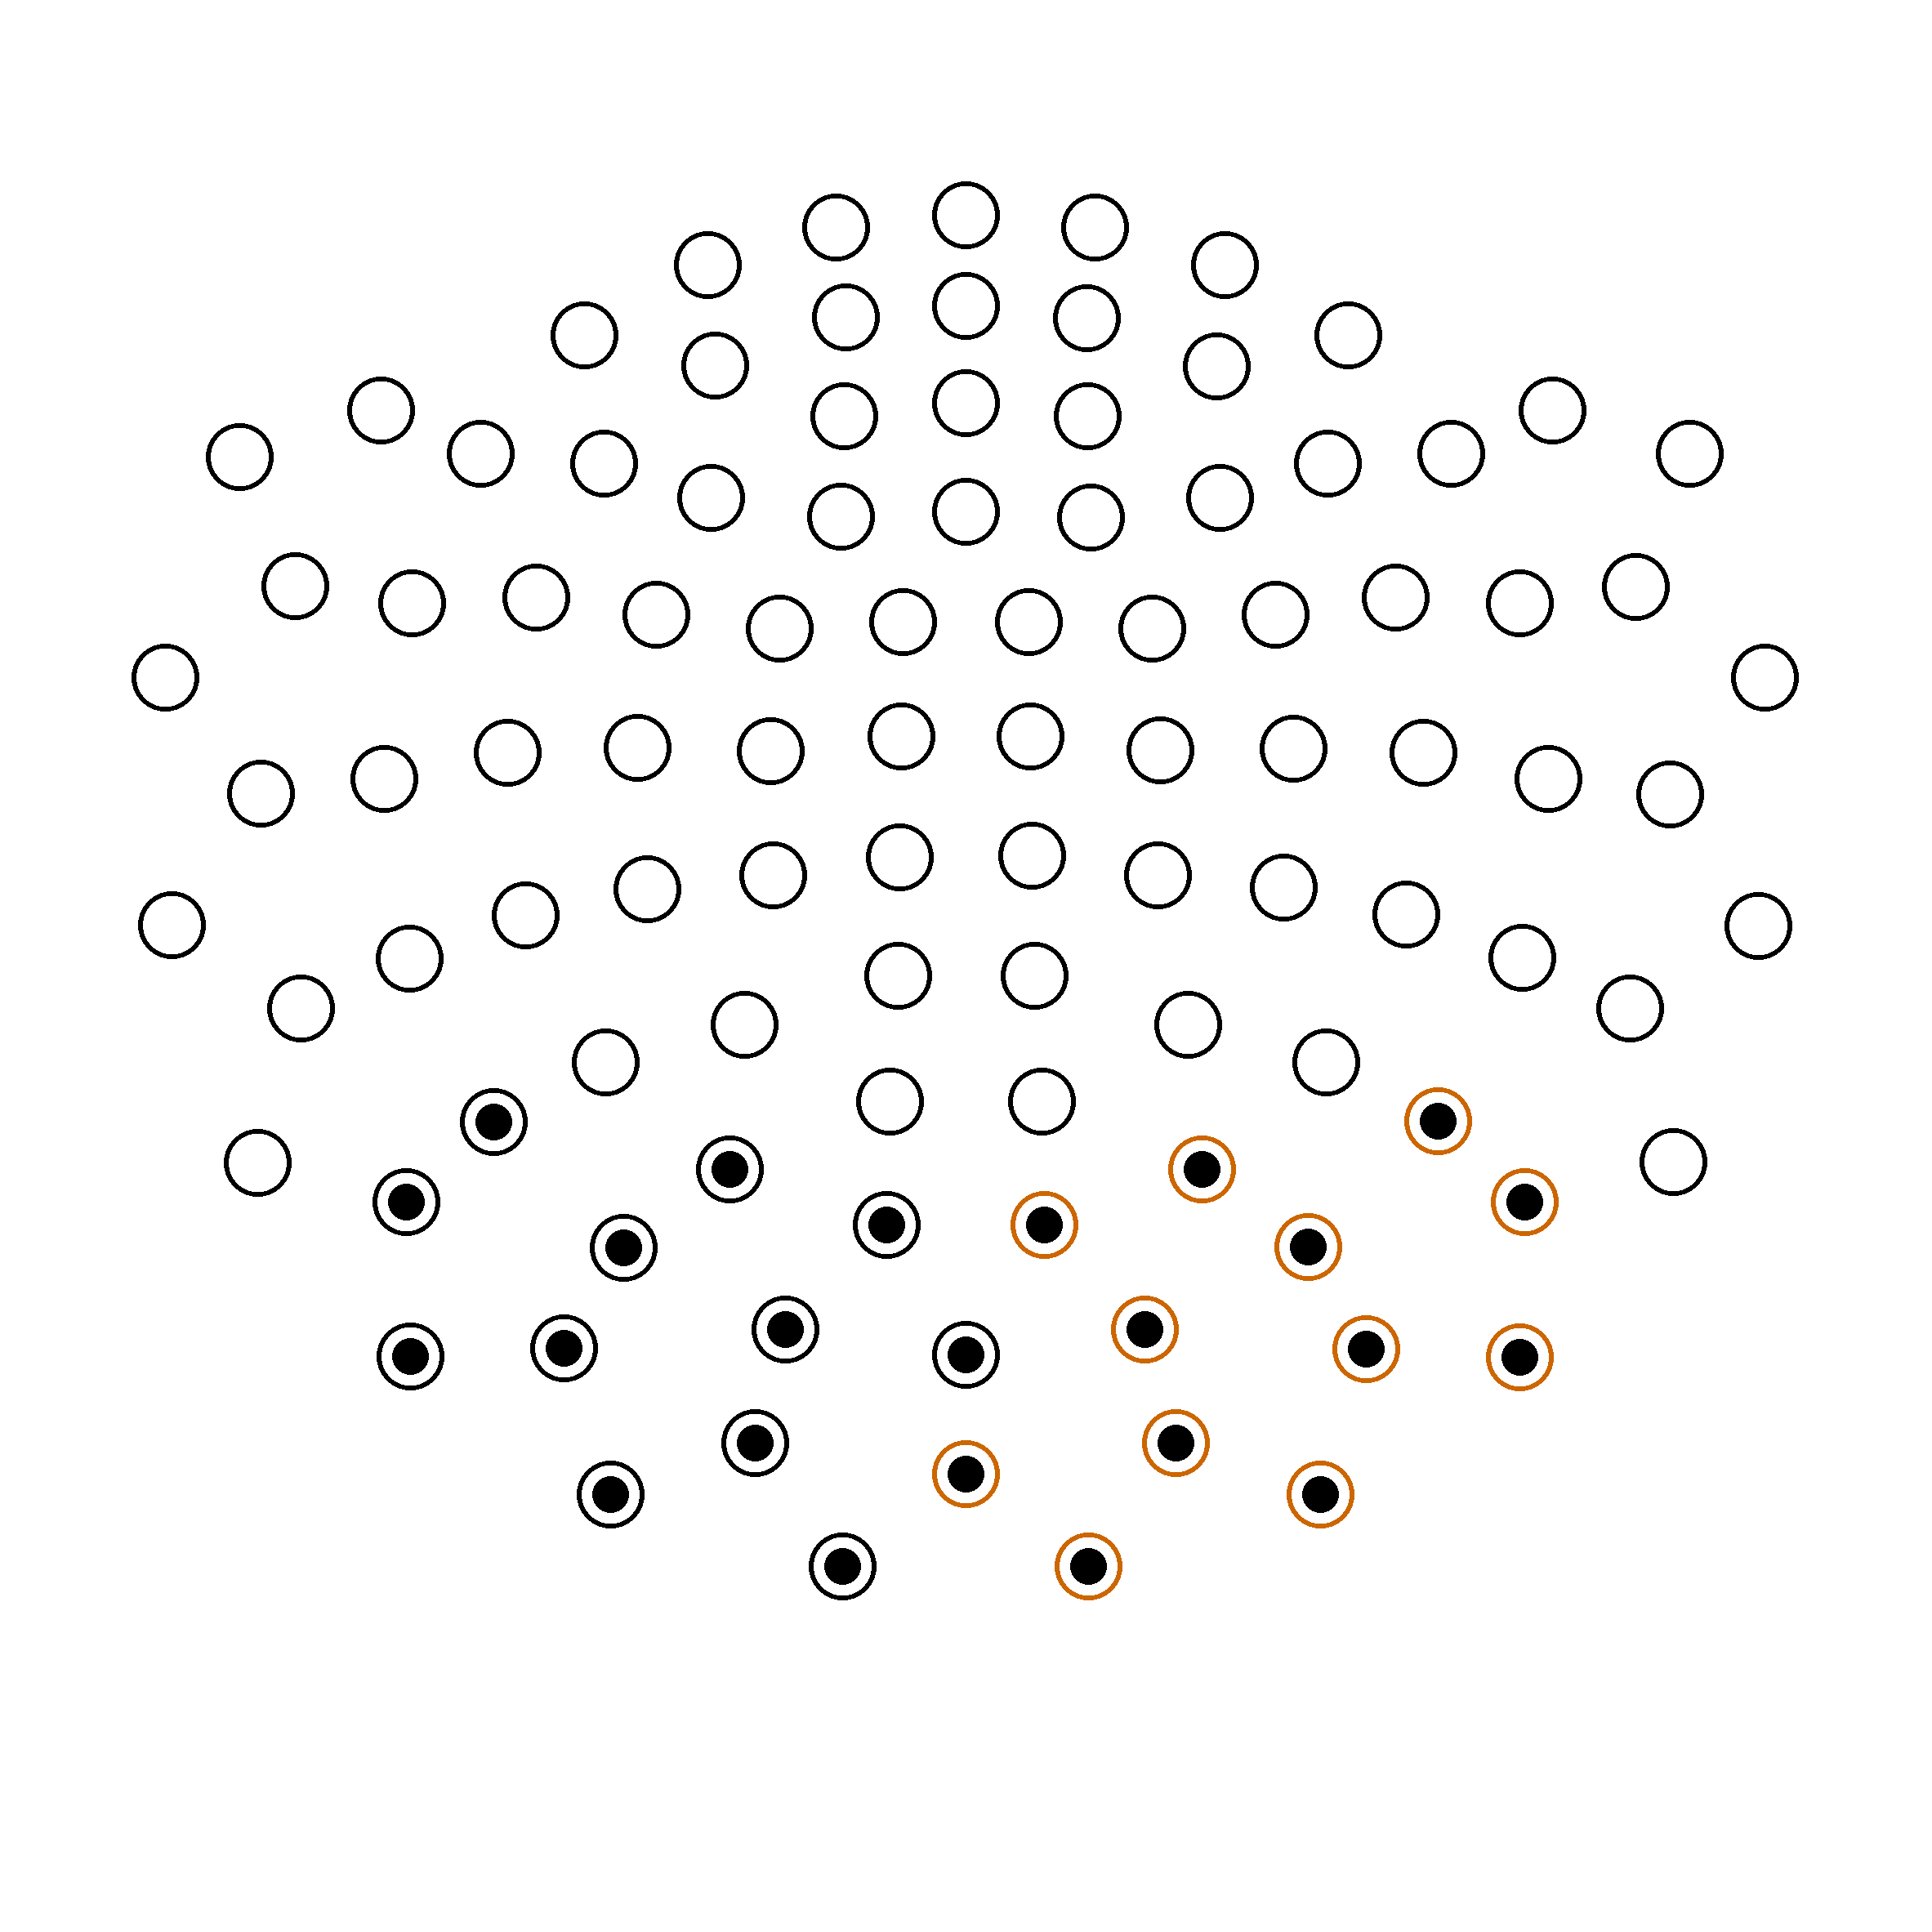
\includegraphics[width=0.24\textwidth]{pics/3_3_occipital_sensors}
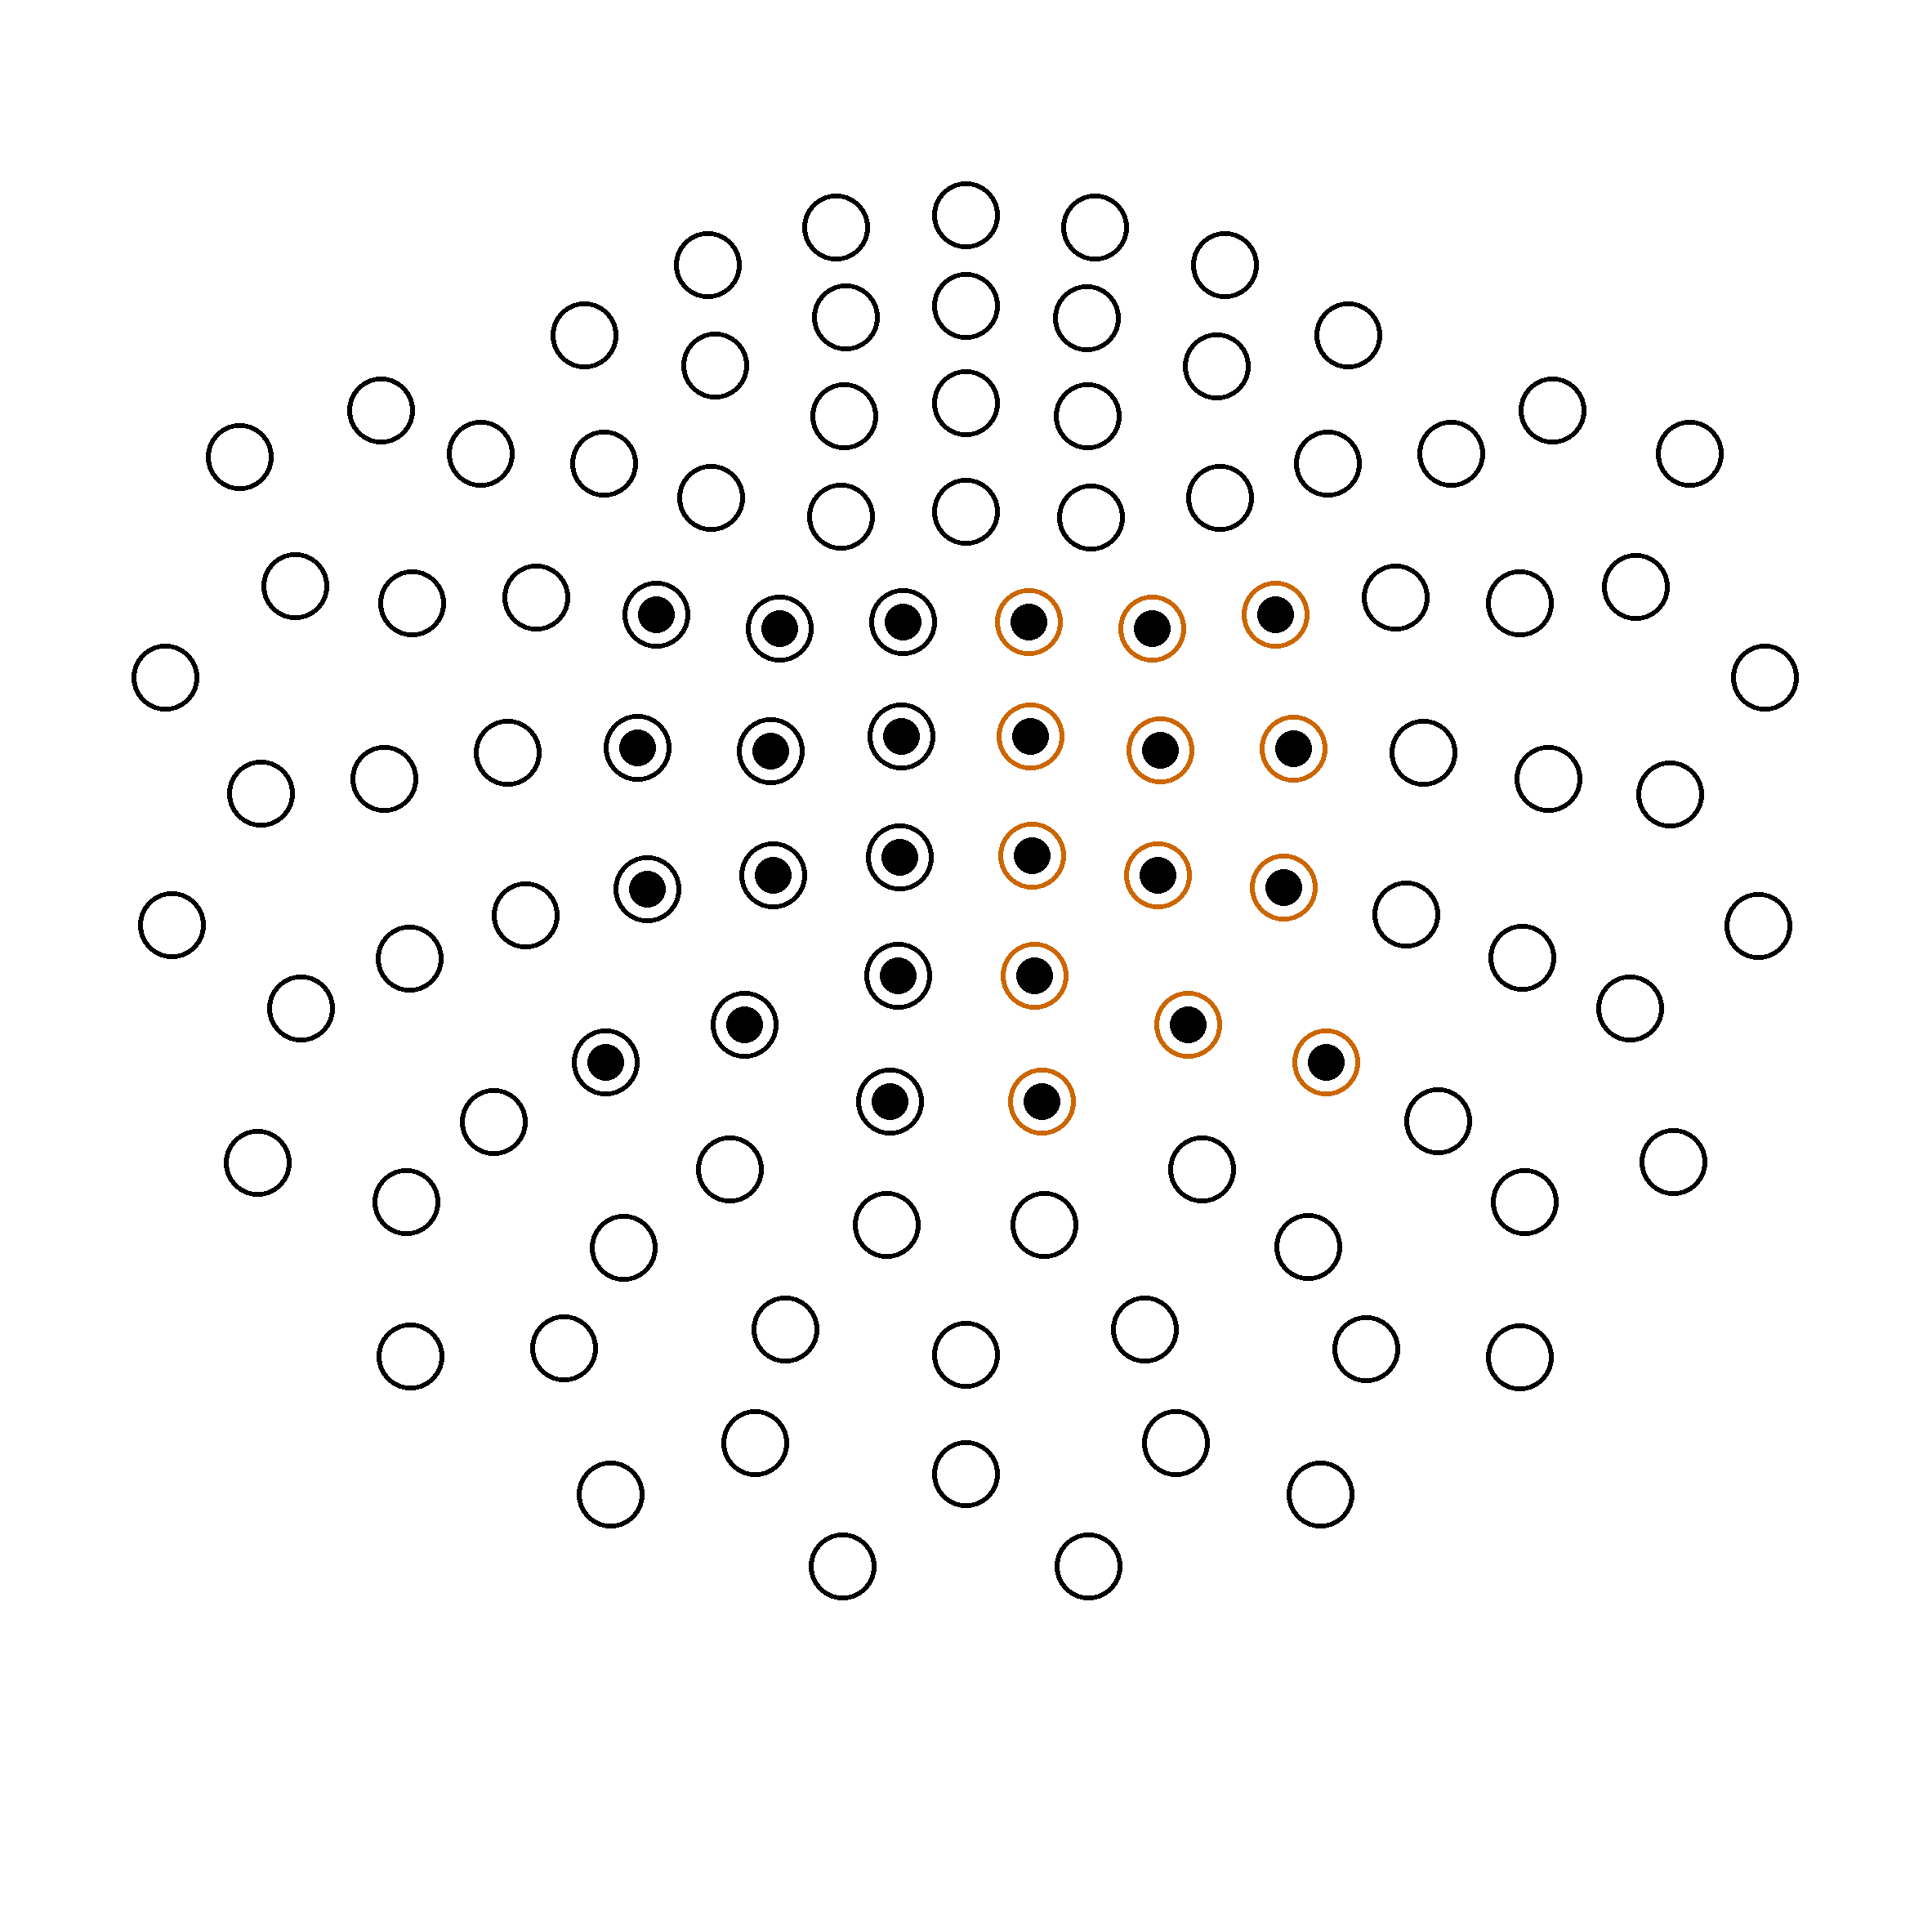
\includegraphics[width=0.24\textwidth]{pics/3_3_parietal_sensors}
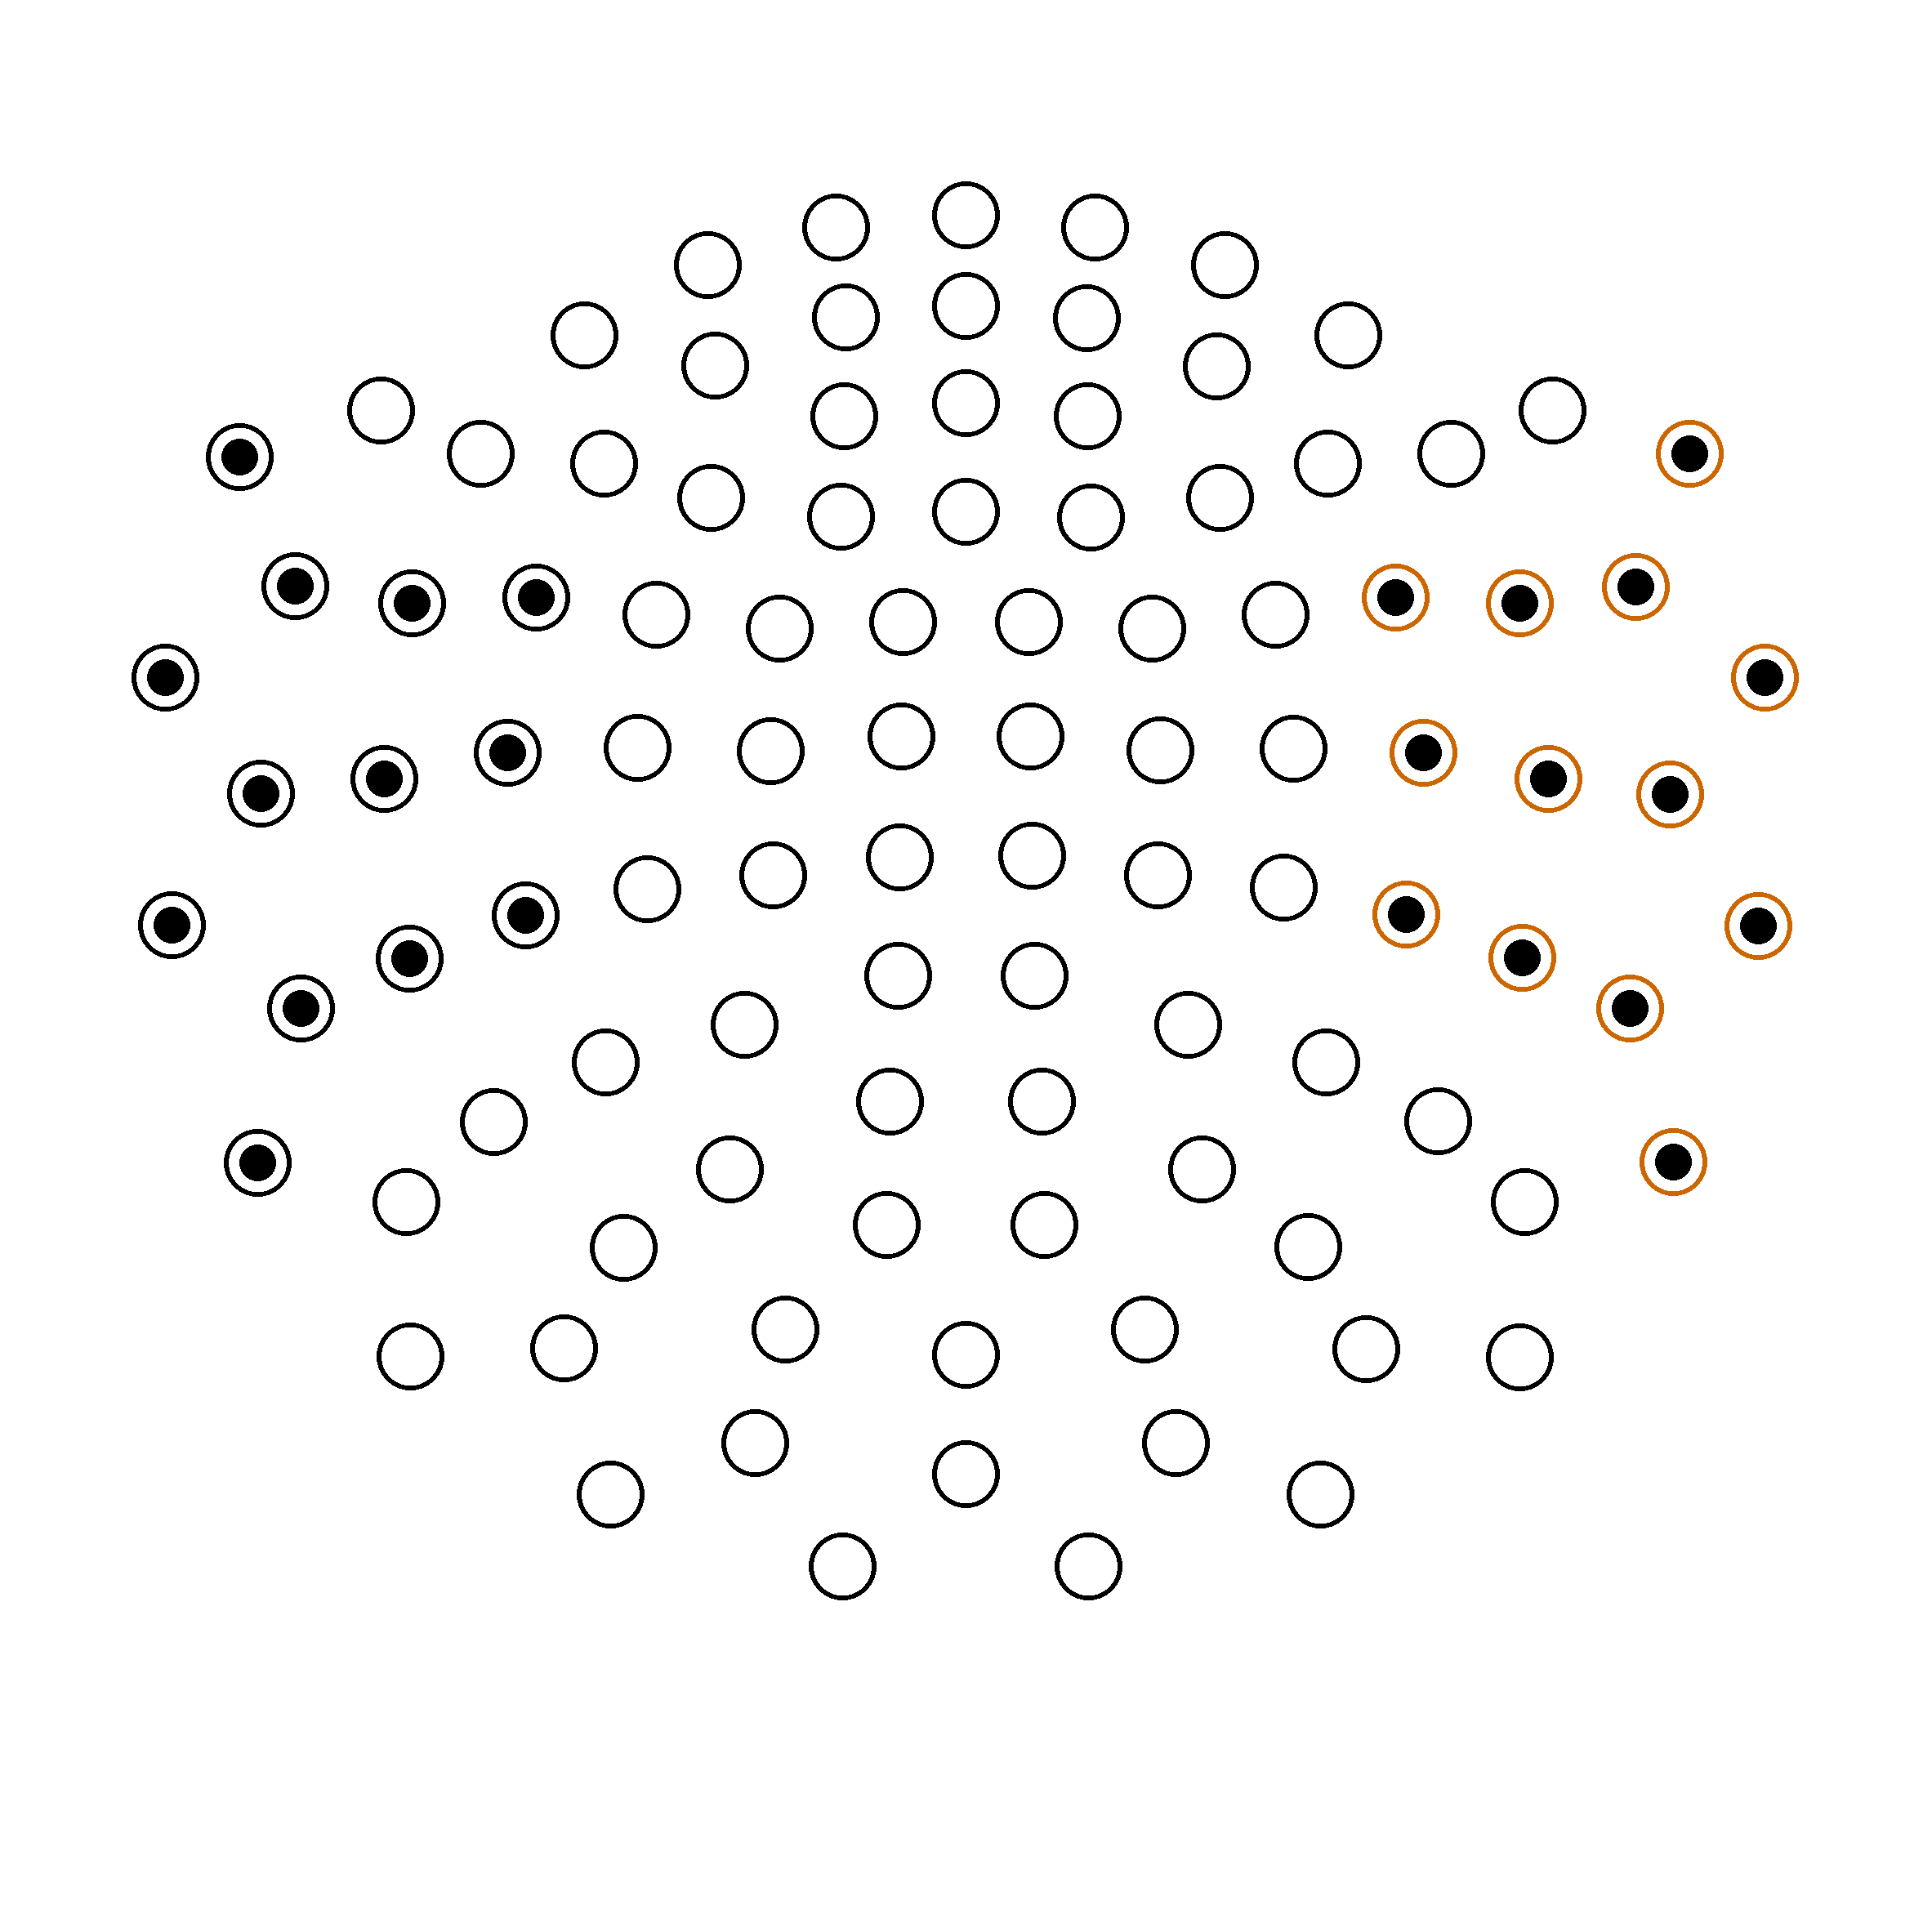
\includegraphics[width=0.24\textwidth]{pics/3_3_temporal_sensors}
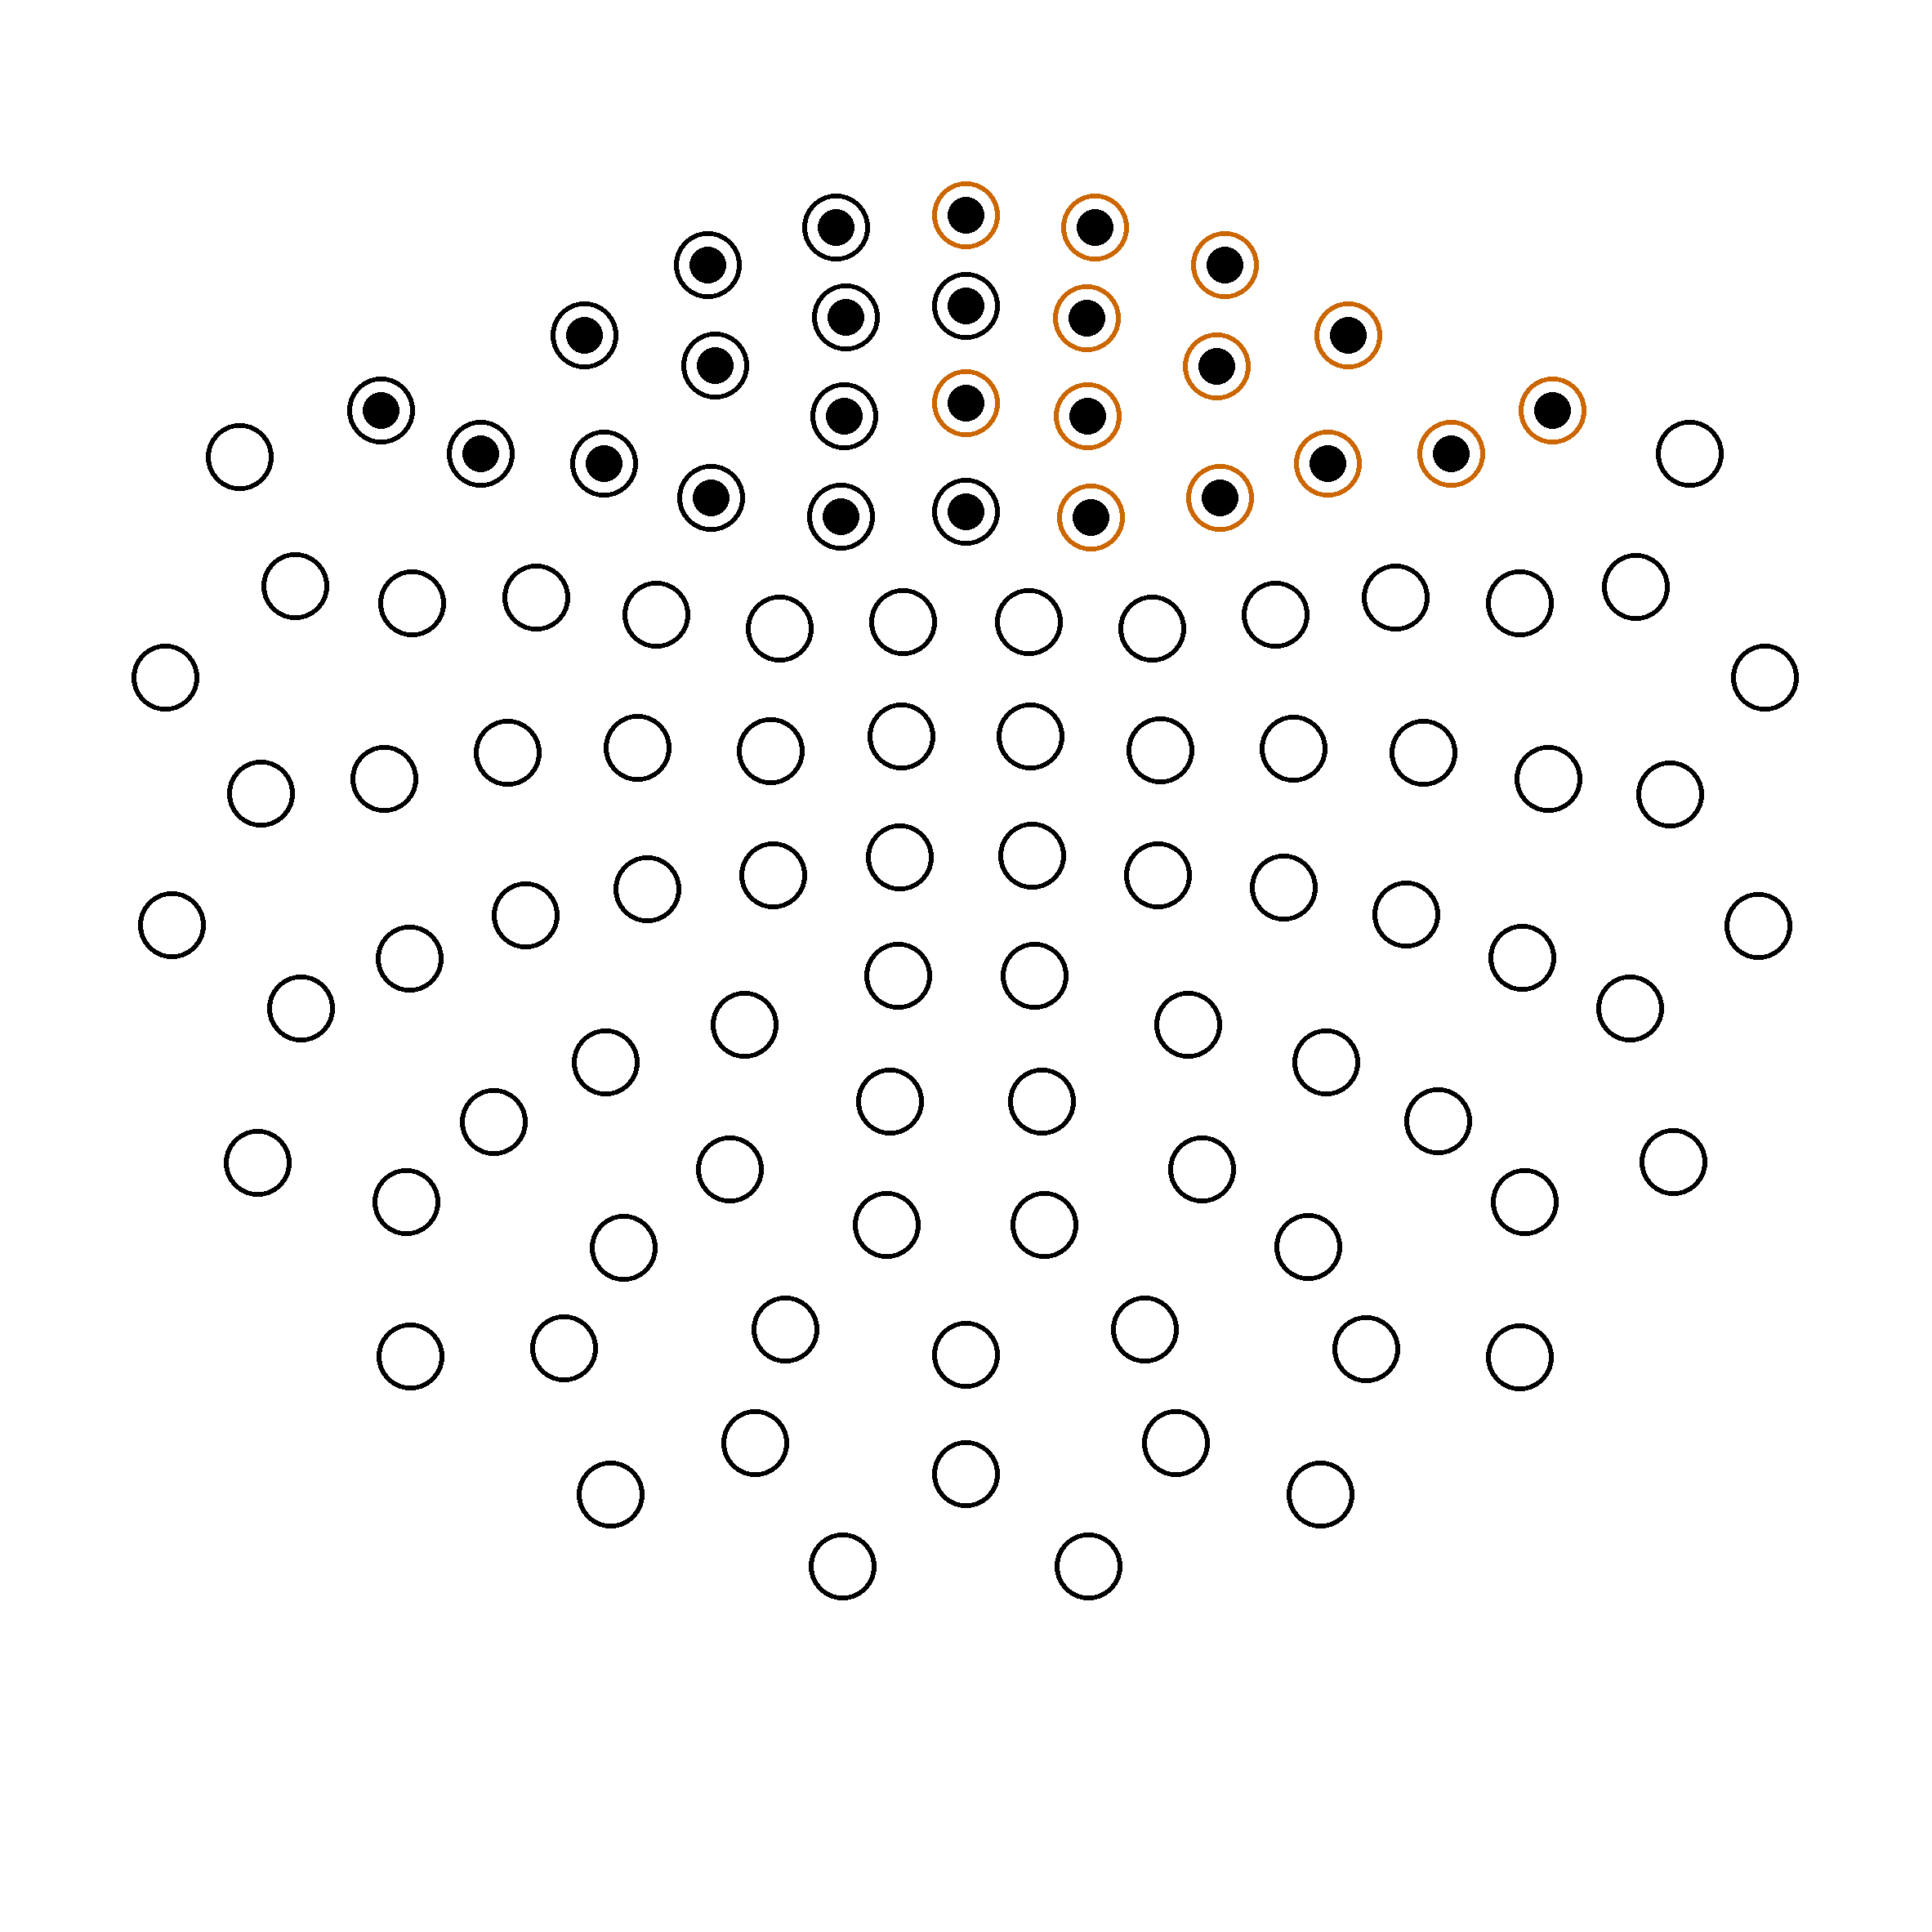
\includegraphics[width=0.24\textwidth]{pics/3_3_frontal_sensors}
\caption{\label{3.3.sensors} Selected channels for each sensor location. From left to right: occipital, parietal, temporal, frontal. The right hemisphere (in red) is also depicted on the right side in each illustration.}
\end{center}
\end{figure}

\subsection{Source space activity}

\paragraph{Anatomical preprocessing}
Cortical reconstruction and volumetric segmentation was performed with the Freesurfer image analysis suite, which is documented and freely available for download online (http://surfer.nmr.mgh.harvard.edu/).
The technical details of these procedures are described in prior publications (Dale et al., 1999; Dale and Sereno, 1993; Fischl and Dale, 2000; Fischl et al., 2001; Fischl et al., 2002; Fischl et al., 2004a; Fischl et al., 1999a; Fischl et al., 1999b; Fischl et al., 2004b; Han et al., 2006; Jovicich et al., 2006; Segonne et al., 2004, Reuter et al. 2010, Reuter et al. 2012).
I followed the recommended processing pipeline ("'recon-all"'), with three optional functions.

First, the option "'-nuintensitycor-3T"' improved brain segmentation accuracy by optimizing the bias field correction \cite{3.3.nuintensity}.

Second, by invoking "'-notal-check"', I skipped the Talairach registration checks.
Talairach registration was prone to failure especially in the infant subjects, and uneccessary for our further processing steps.

Third, I supplied and included T2-weighted MRI datasets with the options "'-T2"' and "'-T2pial"'.
The combination of T1- and T2-weighted images improves tissue differentiation especially around the pia mater, yielding a more accurate cortex segmentation.
This pipeline yielded a continuous, antomically plausible cortical surface in MRI space.


\paragraph{Forward and inverse operator}
For the forward operator, three components were necessary: a source model, a BEM model and a coregistration file.

The cortical surface from Freesurfer was used to construct the source model.
Sources were generated by the MNE function $mne\_setup\_bem$.
The result were 20484 sources (10242 per hemisphere), distributed with approximately equal density over the cortical surface.

The head surface from Freesurfer was used to extract a scalp surface layer.
The BEM was constructed from this scalp layer with the function $mne\_surf2bem$, using the default options.
This function sampled down the original surface to the 4th subdivision of an icosahedron.
The finished BEM consisted of 5140 nodes.

Finally, a coregistration file provided the transformation between MRI space and MEG space.
This coregistration attempted to minimize the distance between digitized head surface points and the head surface extracted from the MRI. 
It was performed for each subject individually using the software $mne\_analyze$.
The initial fit was done manually, with visual error feedback.
The following fine adjustment was performed automatically.
This process was repeated until the average spatial error was less than 2mm.
These three components were assembled into a forward operator by the method $mne\_do\_forward\_solution()$.


For the inverse operator, three components were necessary: the forward model, a noise covariance matrix, and a regularization factor.
Each component was calculated individually for each subject.

The first component, the forward model, was supplied by the previous step.

For the second component, the noise covariance matrix, the 1000ms after visual onset were extracted from each trial.
Then, the covariance matrix was computed from this data with the function $mne.compute\_covariance()$.

The third component, the regularization factor was determined from this noise covariance matrix.
First, only coefficients from gradiometer channels were selected.
Second, these coefficients were transformed with a singular value decomposition.
Third, the upper cutoff was defined as the first value of the transformed coefficients.
Fourth, the index at which the transformed coefficients performed the steepest drop in logarithmic value was determined.
Fifth, this index was defined as the maximum amount of usable dimensions.
Sixth, the lower cutoff was defined as the value at this index, plus 15\%.
Seventh, the regularization factor was computed by dividing the lower cutoff by the higher cutoff.


The inverse operator was computed from these three components by the method \linebreak $mne\_do\_inverse\_operator()$. The regularization factor was supplied with the option \linebreak "'--megreg"'.

\paragraph{Inverse solution}
For determining regional cortical activity, 8 regions needed to be defined: the primary auditory cortex (PAC), the anterior and posterior parts of the superior temporal sulcus (a/pSTS), the anterior and posterior parts of the superior temporal gyrus (a/pSTG), Brodmann area 45 (BA45), Brodmann area 44 (BA44) and the ventral Brodmann area 6 (BA6v).
The regions were spatially defined manually on the cortex of the reference subject.
Freesurfer provided the aparc.a2009s segmentation, which became the basis for this regional selection.
The final regions of interest on the reference brain are visualized in Fig. \ref{3.3.ROI}.
These regions were mapped from the reference cortex onto the cortices of all other subjects during the next step.

\begin{figure}[h]
\begin{center}
\vspace{7mm}
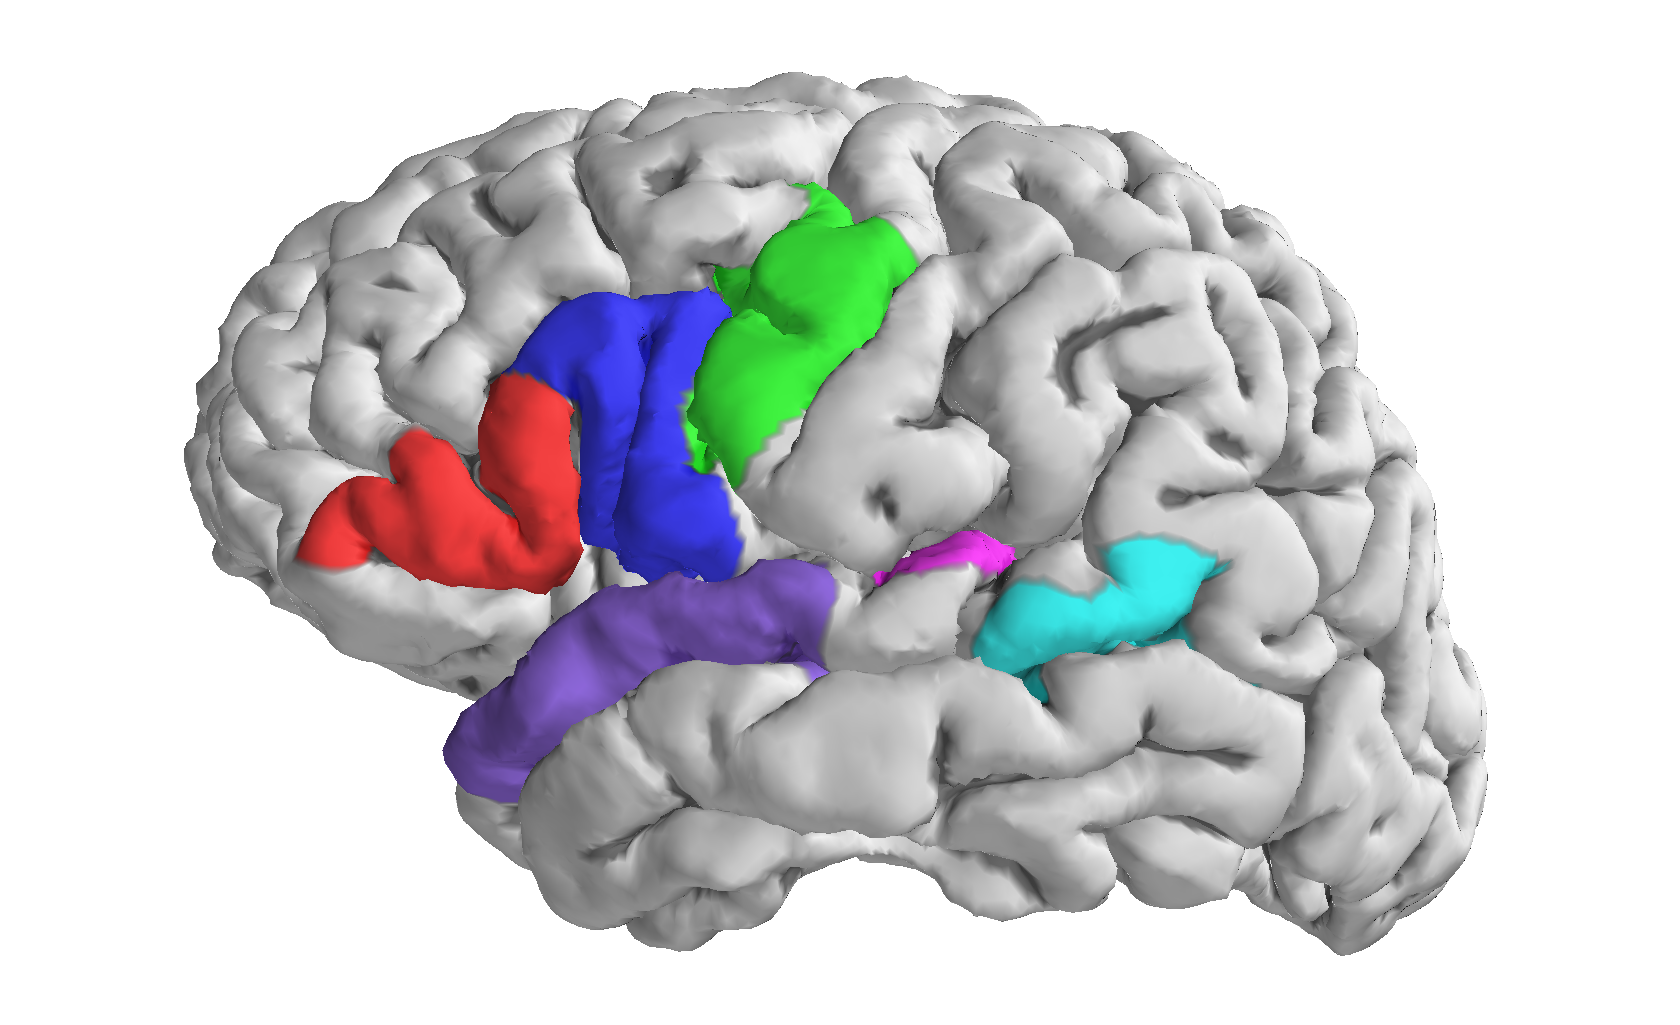
\includegraphics[width=0.49\textwidth]{pics/dh55a-pial-lh}
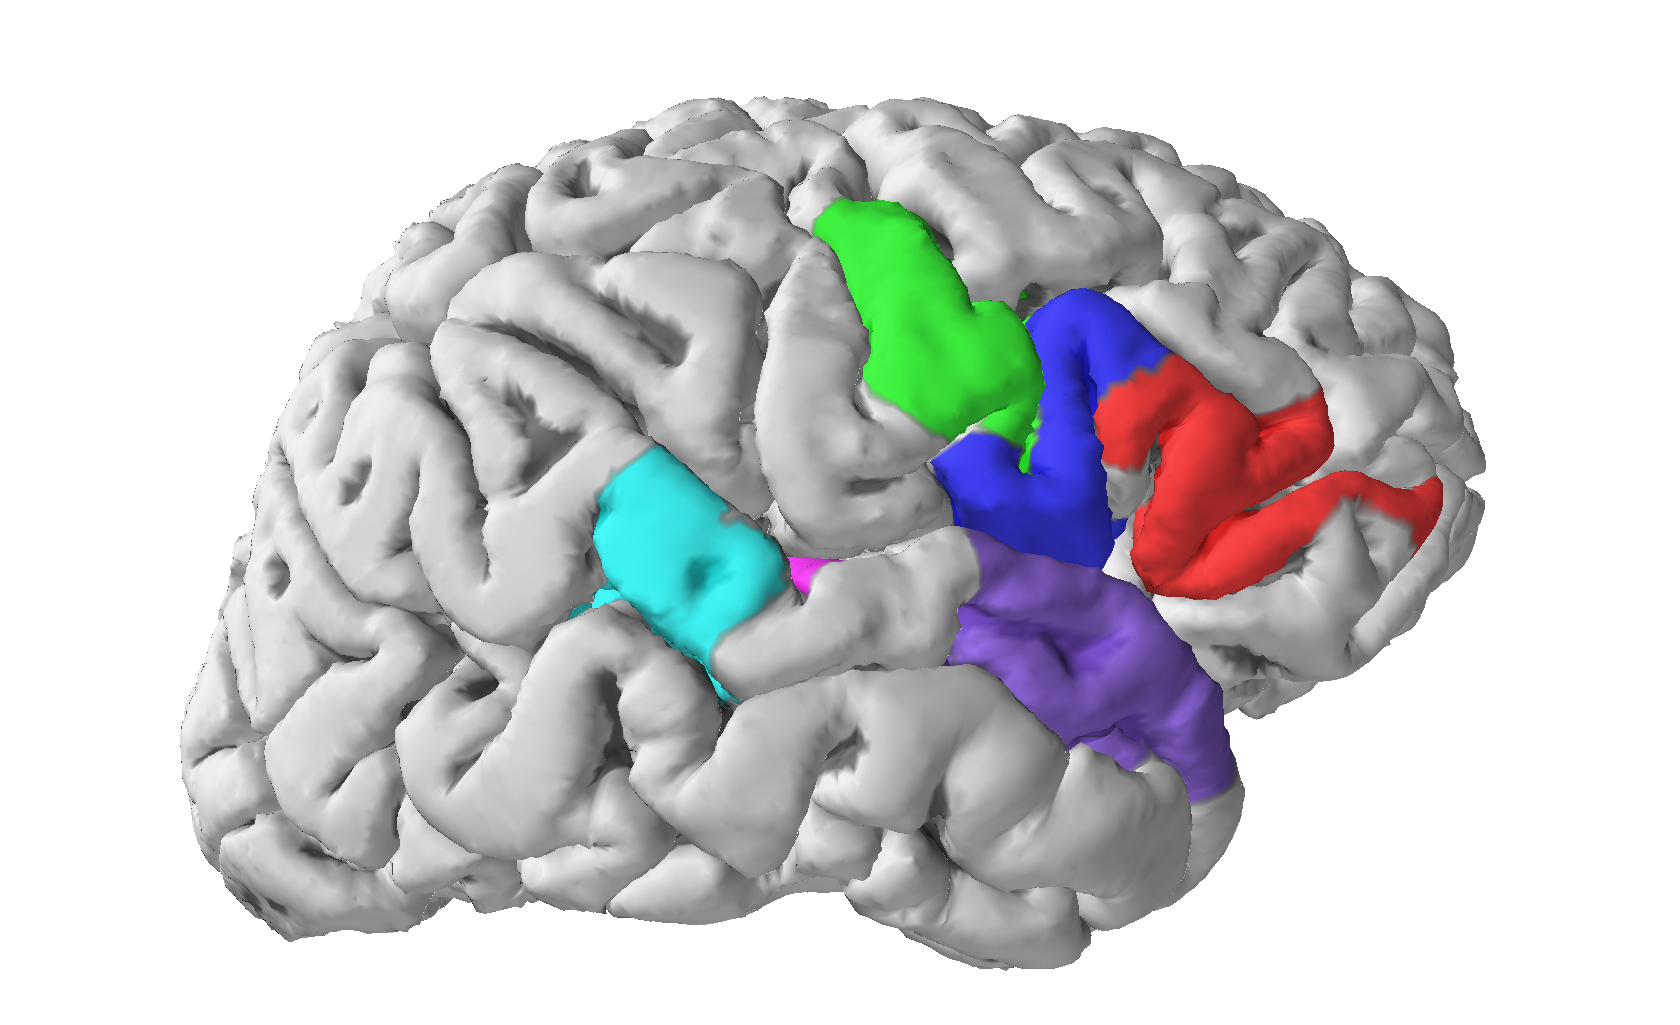
\includegraphics[width=0.49\textwidth]{pics/dh55a-pial-rh}
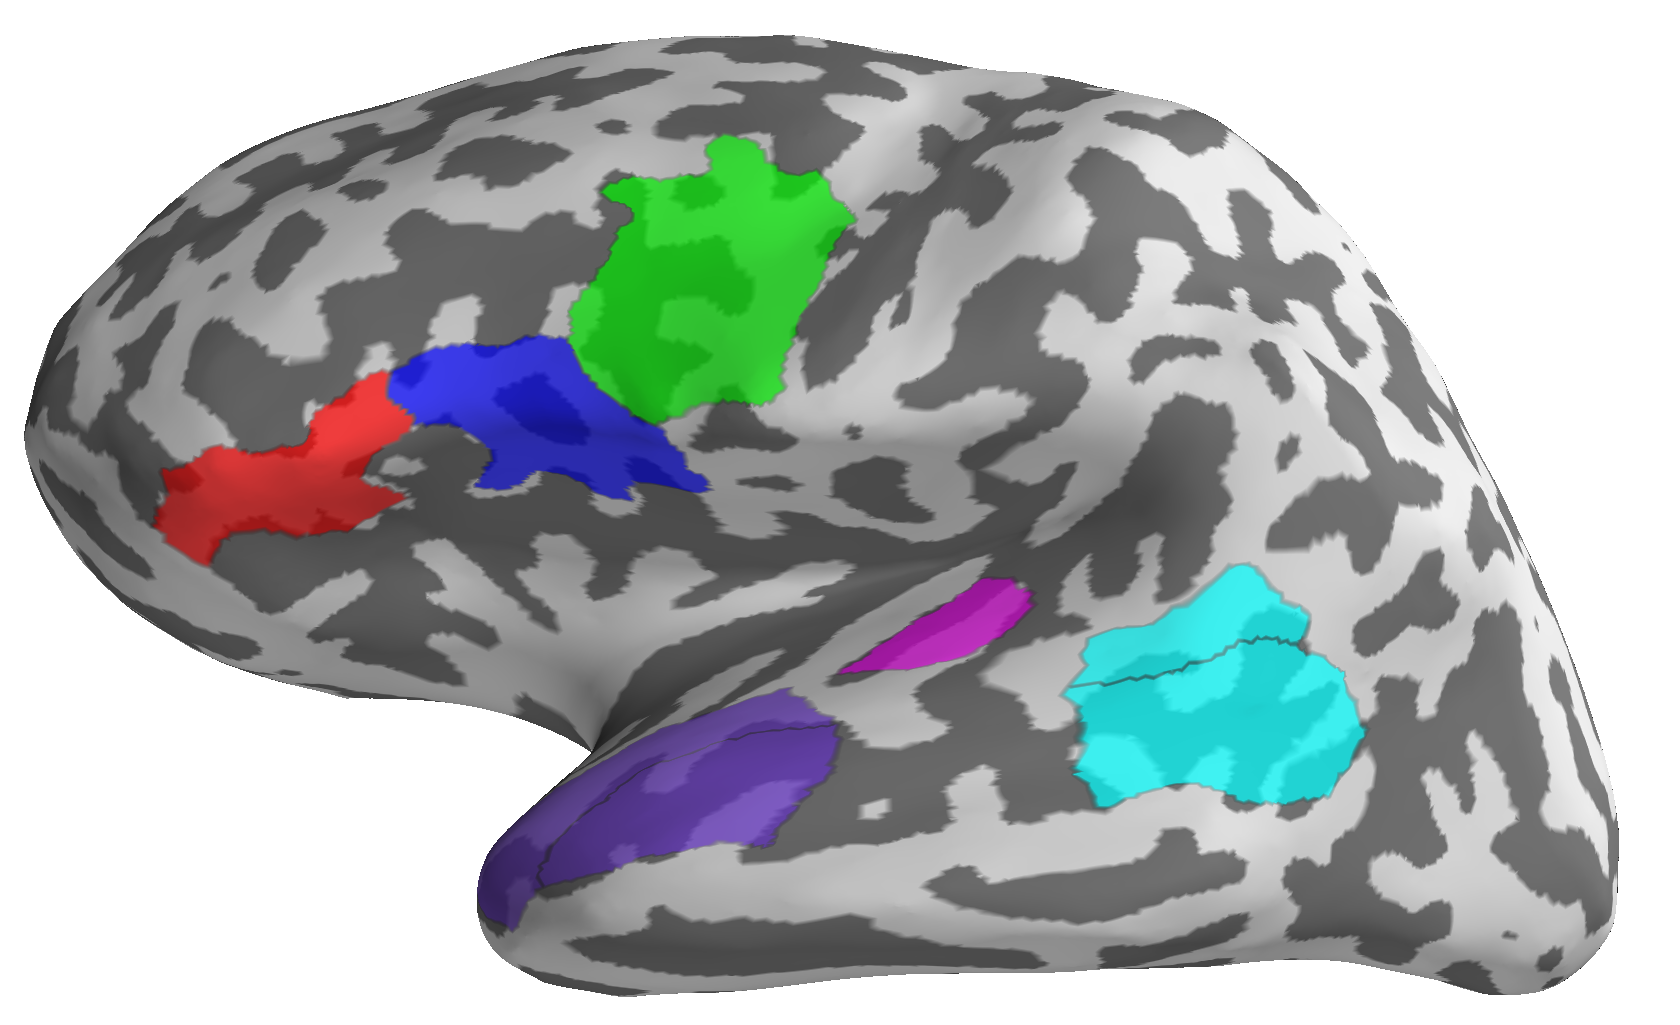
\includegraphics[width=0.49\textwidth]{pics/dh55a-inflated-lh}
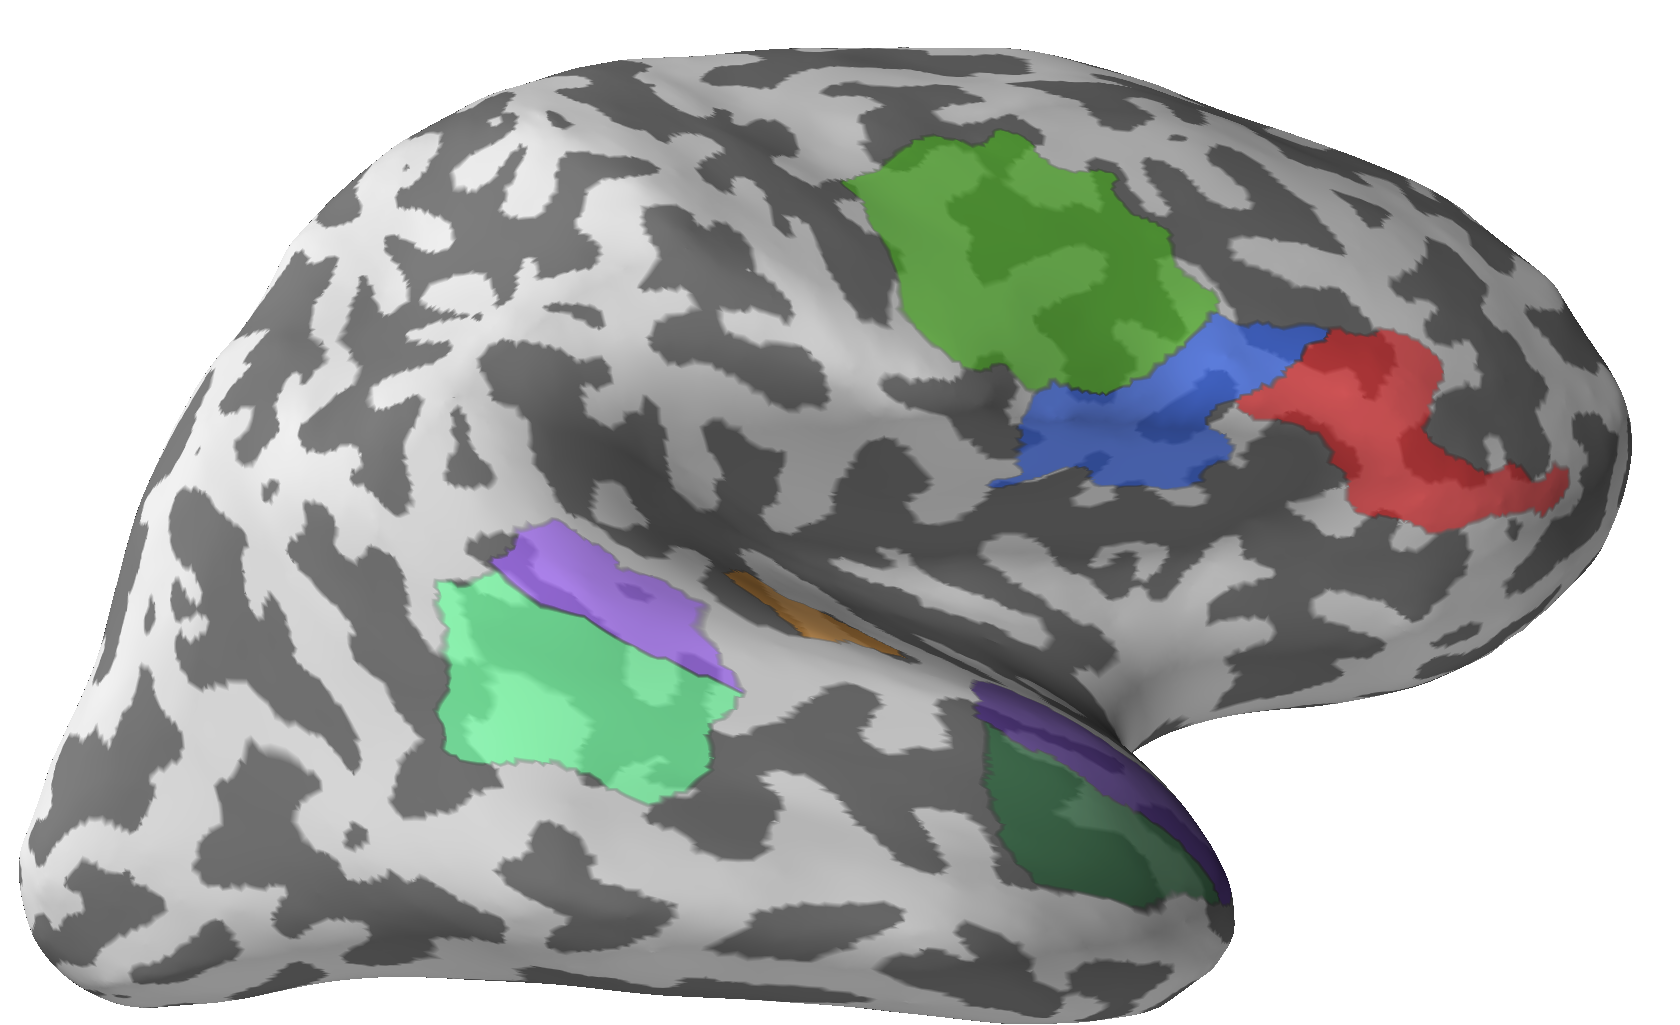
\includegraphics[width=0.49\textwidth]{pics/dh55a-inflated-rh}
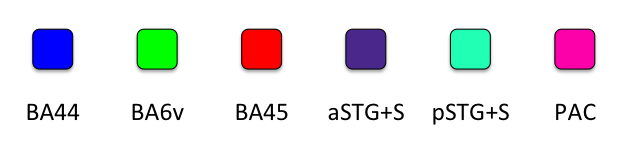
\includegraphics[width=0.75\textwidth]{pics/3_3_ROIlegend}
\caption{\label{3.3.ROI} Selected regions of interest on the reference brain. Top: selected regions on the folded cortex. Bottom: selected regions on the inflated cortex.}
\end{center}
\end{figure}

The inverse operator was then used to calculate inverse solutions from MEG sensor data.
Inverse solutions were calculated for each time point, region, trial and subject individually.
The process was performed by the function $mne.minimum\_norm.apply\_inverse\_epochs()$, with sLORETA as the inverse method.
The option "'pick\_ori=normal"' ensured that currents leaving and entering the cortex were designated positive and negative, respectively.
Due to the combination of passive and active noise reduction and artifact suppression, I assumed a fairly high signal-to-noise-ratio (SNR) of 100:1 for each individual source.
The regularization factor was estimated by $\frac{1}{SNR} = 10^{-4}$.
The result was a series of activation patterns within each region.
Finally, the mean of regional node activity was calculated for each time point, region, trial and subject.


The resulting localized activity was again subjected to a cluster analysis.
Extracted trials were split into a 4 parts (2 groups x 2 conditions).
The two groups were evaluated separately.
Trials contained average data from six regions (PAC, aSTS+G, pSTS+G, BA44, BA45 and BA6v).
Clusters were determined with the MNE function $stats.permutation\_cluster\_test()$ \cite{3.3.clustertest}.
The function was run with 2500 permutations, and an t-threshold of 2.0.

For visualization purposes, grand average activity was calculated for each cortical region, group and condition.


% \subsection{Interaction analysis}

% The TRENtool software was used for exploring transfered entropy between cortical areas.
% - Role of embedding, Ragwitz optimization
% - statistical tests between conditions and multiple comparisons